\documentclass{article}
\usepackage[margin=1.25in]{geometry}

% Recommended, but optional, packages for figures and better typesetting:
\usepackage{microtype}
\usepackage{graphicx}
% \usepackage{subfigure}
\usepackage{wrapfig}
\usepackage{caption}
\usepackage{float}
\usepackage{subcaption}
\usepackage{booktabs} % for professional tables
\usepackage[shortlabels]{enumitem}
\usepackage{parskip}

\usepackage{hyperref}
\usepackage{natbib}


\usepackage{mymathstyle}

% For theorems and such
\usepackage{amsmath}
\usepackage{amssymb}
\usepackage{mathtools}
\usepackage{amsthm}

% if you use cleveref..
\usepackage[capitalize,noabbrev]{cleveref}

%region custom commands
\newcommand{\softreliprod}[3]{\left\langle #1, #2 \, \vert \, #3 \right\rangle_\mathrm{rel}}
\newcommand{\reliprod}[2]{\left\langle #1, #2 \right\rangle_\mathrm{rel}}
% \let\phi\varphi
%endregion


% Todonotes is useful during development; simply uncomment the next line
%    and comment out the line below the next line to turn off comments
% \usepackage[disable,textsize=tiny]{todonotes}
\usepackage[textsize=tiny]{todonotes}

\title{Learning Hierarchical Relational Representations through \\ Relational Convolutions}
\author{Awni Altabaa \and John Lafferty}
\begin{document}
\maketitle

\begin{abstract}
    A maturing area of research in deep learning is the study of architectures and inductive biases for learning representations of relational features. In this paper, we focus on the problem of learning representations of \textit{hierarchical} relations, proposing an architectural framework we call ``relational convolutional networks''. Given a sequence of objects, a ``multi-dimensional inner product relation'' module produces a relation tensor describing all pairwise relations. Graphlet filters, analogous to filters in convolutional neural networks, represent a template for the pattern of relations in patches of the input (i.e., groupings of objects). By matching the graphlet filters against different groups of objects, a ``relational convolution'' layer transforms the relation tensor into a sequence of new objects, each describing the relational pattern within a group of objects at the previous layer. Repeating this yields representations of higher-order, hierarchical relations. We present the motivation and details of the architecture, together with a set of experiments to demonstrate how relational convolutional networks can provide an effective framework for modeling relational tasks that have hierarchical structure.
\end{abstract}

\section{Introduction}\label{sec:intro}


%\begin{itemize}
%    \item The importance of relational learning; lots of references.
%    \item We propose a framework analogous to CNNs, but for relational learning
%    \item Advantages: modularity, compositionality, hierarchical.
%    \item Experiments showing advantages over existing frameworks. 
%    \item Main contribution: Framework for relational learning that shares the %strengths of CNNs for relational learning
%\end{itemize}

Modeling of relations between objects is important to a range of machine learning problems. For instance, an image analysis application might rely on comparing objects in terms of relations that extract color, size, or texture features; a natural language task may use relations that are based on syntactic or semantic features of pairs of words. While some machine learning tasks are ``purely relational'' and rely exclusively on identification and processing of relational information, others combine extraction of relations with function approximation.

To enable efficient learning of relational information, it is important to explore learning architectures that support processing of relations in a natural, expressive, and efficient manner. In this paper we propose a framework we call ``relational convolution networks.'' Our framework provides for relational representation learning what standard convolutional neural networks provide for typical image processing applications---a natural, expressive architecture for extracting hierarchical features of the raw data that can be used for building flexible prediction algorithms.

A schematic of the proposed architecture to support hierarchical relational learning is shown in Figure~\ref{fig:relconv_architecture}. Beginning with embeddings of objects, a multi-head relation module takes a sequence of embedded objects as input and produces a tensor that represents the relations between each pair of objects. The relational convolution layer then transforms the relation tensor into a sequence of new objects, each describing the relations within some group of objects at the previous layer.  An important component of the architecture is to use ``graphlets'' to carry out the relational convolution operation over groupings of the objects. Analogous to filters in CNNs, relational graphlets form a template of relations between subsets of objects against which the relation tensor is compared. The next layer receives this sequence of new objects as input and again models the relations within it. Thus, each layer computes relational features of a higher order---that is, relations on relations. This is analogous to the manner in which convolutional layers in a CNN can be composed to construct a chain of feature maps.

In a series of experiments, we show how relational convolutional neural networks provides an effective framework (and inductive bias) for relational learning. We first carry out experiments on ``relational games" proposed as a benchmark for relational reasoning by~\citep{shanahanExplicitlyRelationalNeural}. This consists of a suite of binary classification tasks for identifying abstract relational rules between a set of objects represented as images. We next carry out experiments on a version of the SET game, which requires processing of  higher-order relations between multiple attributes on a set of cards. For both tasks, relational convolutional networks are able to achieve more sample efficient learning compared to Transformers, as well as other architecture that have been specifically developed for relational learning.

\begin{wrapfigure}{R}{0.5\textwidth}
    \centering
    \includegraphics[width=.5\textwidth]{figs/relconv_architecture.pdf}
    \caption{Proposed architecture for relational convolutional networks. Hierarchical relations are modeled by iteratively computing pairwise relations between objects and convolving the resultant relation filter with graphlet filters representing templates of relations between subsets of objects.}
    % At each layer, the multi-head relation module takes a sequence of objects as input and produces a relation tensor representing the relations between each pair of objects. The relational convolution layer then transforms the relation tensor into a sequence of objects each describing the relations within some group of objects at the previous layer. The next layer receives this sequence of objects as input and again models the relations within it. Thus, each layer computes relational features of a higher order (i.e., relations on relations). \textit{Legend}: $d_l$ represents the dimension of the objects at layer $l$; $z_i^{(l)}$ is the $i$th object at the $l$th layer; $R^{(k)}$ is the relation tensor at layer $l$; $r_l$ is the dimension of the relations at layer $l$; $n_l$ is the number of objects at layer $l$. \awni{can we cut down on the caption a bit for space?} \awni{should I make the modules different colors?}}\label{fig:relconv_architecture}
\end{wrapfigure}

\subsection{Related Work}

Several previous works have considered the design of machine learning architectures which support the representation of relational information, in various forms~\citep{battagliaRelationalInductiveBiases2018,palmRecurrentRelationalNetworks2018,zhangRAVENDatasetRelational2019}.

\textbf{Graph Neural Networks.} Graph neural networks (GNNs) are a class of neural network architectures which operate on graphs and process ``relational'' data~\citep{niepertLearningConvolutionalNeural2016,kipfSemiSupervisedClassificationGraph2017,schlichtkrullModelingRelationalData2017,velickovicGraphAttentionNetworks2017,kipfNeuralRelationalInference2018}. A defining feature of the GNN model is its use of a form of neural message-passing, wherein the hidden representation of a node is updated as a function of the hidden representations of its neighbors~\citep{gilmerNeuralMessagePassing2017}. Typical examples of tasks which GNNs are applied to include node classification, graph classification, and link prediction~\citep{hamiltonGraphRepresentationLearning2020}. %This is a very general model which includes as a special case convolutional neural networks, where the graph is a grid, and Transformers, where the graph is a complete graph and the message-passing function is a convex sum of the neighbors' representations. In our experiments, we compare to Transformers as a representative of the GNN model.

In GNNs, the `relations' are given to the model via edges in a graph. In contrast, our architecture, as well as the explicitly relational architectures described below, operate on collections of objects without any relations given as input. Instead, such relational architectures must infer the relevant relations from the objects themselves. Still, graph neural networks can be applied to relational tasks by passing in the collection of objects along with a complete graph. A Transformer Encoder can be thought of as a special case of this architecture.%, and hence is the representative baseline we compare against in our experiments.

\textbf{Attention as modeling relations} Several works have proposed architectures with the ability to model relations by incorporating an attention mechanism~\citep{vaswani2017attention,locatelloObjectCentricLearningSlot2020,santoroRelationalRecurrent2018,zambaldiDeepReinforcementLearning2018,velickovicGraphAttentionNetworks2017}. Attention mechanisms model relations between objects implicitly as an intermediate step in a form of neural message-passing in order to update the representation of each object as a function of its context.

\textbf{Emerging literature on ``explicitly relational'' architectures.} There exists a growing literature on neural architectures which aim to explicitly model relational information between objects. An early example is~\citep{santoroSimpleNeural2017}.~\citet{shanahanExplicitlyRelationalNeural} proposes the PrediNet architecture, which aims to learn relational representations which are compatible with predicate logic.~\citet{webbEmergentSymbols2021} proposes ESBN, a recurrent neural network augmented with external memory with a memory-write operation which factors representations into `sensory' and `relational'.~\citet{kergNeuralArchitecture2022} proposes CoRelNet, a simple architecture based on `similarity scores' which aims to distill the relational inductive biases discovered in previous work into a minimal architecture.~\citet{altabaaAbstractorsTransformer2023} explored relational inductive biases in the context of Transformers, and proposed a view of relational inductive biases as a type of selective ``information bottleneck'' which disentangles relational information from object-level features.~\citet{webbRelationalBottleneckInductive2023} provides a cognitive science perspective on this idea, arguing that a relational information bottleneck may be a mechanism for abstraction in the human mind.% and brain.

We aim to contribute to this literature by proposing a framework for learning hierarchical relational representations through a natural compositional architecture. %in a natural, interpretable, sample-efficient, and parameter-efficient manner.

\section{Multi-dimensional inner product relation module}\label{sec:mhr}

% AWNI: TODO: revise this section  and re-write?

A relation function is a function which maps a pair of objects $x, y \in \calX$ to a vector representing the relation between the two objects. For example, a relation may represent the information ``$x$ has the same color as $y$'', ``$x$ is larger than $y$'', and ``$x$ is to the left of $y$''. In principle, this can be modeled by an arbitrary learnable function on the concatenation of the two objects' representations. For example,~\citep{santoroSimpleNeural2017} models relations by MLPs applied to the concatenation of pairs of objects. While this approach may work in some cases, it is missing some crucial inductive biases. In particular, there is no constraint that the learned pairwise function is in fact \textit{relational}---it may just as well represent non-relational information like ``$x$ is bright'' and ``$y$ is small.''%, as opposed to relational information like ``$x$ is larger than $y$''.

Recent work on relational representation has explored using \textit{inner products} to model relations between objects~\citep{webbEmergentSymbols2021, kergNeuralArchitecture2022, altabaaAbstractorsTransformer2023}. The advantage of such an approach is that it provides added pressure to learn explicitly relational representations, disentangling relational information from attributes of individual objects. In particular, it induces a geometry on the object space $\calX$ which allows objects to be described in relation to each other. For example, in the symmetric case, the inner product $\iprod{\phi(x)}{\phi(y)}$ induces a metric on $\calX$. In fact, the relation $\iprod{\phi(x)}{\phi(y)}$ attaches well-defined notions of distance, angles, and orthogonality to the space $\calX$.

More generally, we can allow for multi-dimensional relations by having multiple encoding functions, each extracting a feature to compute a relation on. Furthermore, we can allow for asymmetric relations by having different encoding functions for each object. Hence, we model relations by,
\begin{equation}\label{eq:relation_function}
    r(x, y) = \paren{
        \iprod{\phi_1(x)}{\psi_1(y)},\, \ldots,\, \iprod{\phi_{d_r}(x)}{\psi_{d_r}(y)}} \in \reals^{d_r},
\end{equation}
where $\phi_1, \psi_1, \ldots, \phi_{d_r}, \psi_{d_r}$ are learnable functions. For each dimension of the relation function, the maps $\phi_k, \psi_k$ extract a particular attribute of the objects which is then compared by the inner product.

The intuition is that the encoder extracts, or `filters' out, a particular attribute of the object and the inner products computes similarity across that attribute. A relation, in this sense, is similarity across a particular attribute. In the asymmetric case, the attributes extracted from the two objects are different, resulting in an asymmetric relation where a particular attribute of the first object is compared with a different attribute of the second object. This can model relations of the form "object 1 is light and object 2 is dark", for example (an antisymmetric relation).

To promote weight sharing, we can have one common non-linear map $\phi$ across all dimensions along with different linear maps for each object and each dimension of the relation. That is,
\begin{equation}\label{eq:relation_function_lin_proj}
    r(x, y) = \paren{\iprod{W_1^{(1)}\phi(x)}{W_2^{(1)}\phi(y)},\, \ldots,\, \iprod{W_1^{(d_r)}\phi(x)}{W_2^{(d_r)}\phi(y)}},
\end{equation}
where the learnable parameters are $\phi$ and $W_1^{(k)}, W_2^{(k)}, k \in [d_r]$. $\phi: \calX \to \reals^{d_\phi}$ may be an MLP, for example, and $W_1^{(k)}, W_2^{(k)}$ are $d_{\mathrm{proj}} \times d_\phi$ matrices. The class of functions realizable by~\Cref{eq:relation_function_lin_proj} is the same as~\Cref{eq:relation_function} but enables greater weight sharing.

The ``Multi-dimensional Inner Product Relation'' (MD-IPR) module receives a sequence of objects $x_1, \ldots, x_n$ as input and models the pairwise relations between them by~\Cref{eq:relation_function_lin_proj}, returning an $n \times n \times d_r$ relation tensor, $R[i,j] = r(x_i, x_j)$, describing the relations between each pair of objects.

% removed for now.
% \subsection{Universal approximation of inner product relations}
% \awni{todo---post to arxiv and add citation. Also, is statement as a theorem necessary, or should we just state the result in text?}

\citep{arxivInnerprodUnivApprox} analyzes the function class of relation functions on $\calX \times \calX$ realizable by inner products of neural network transformations of the form $\iprod{\phi(x)}{\psi(y)}$. The result implies that when $\phi_i, \psi_i$ are multi-layer perceptrons, $r(x,y)$ in~\Cref{eq:relation_function} can approximate any continuous function from $\calX \times \calX$ to $\reals^{d_r}$ uniformly and with arbitrary precision, provided that $\calX$ is a compact subset of euclidean space.

\begin{theorem}[Theorem 3.1 in~\citep{arxivInnerprodUnivApprox}]
    Suppose $\calX$ is a compact subset of euclidean space. Consider the relation model,
    \begin{equation*}
        \hat{r}(x, y) := \paren{\iprod{\phi_\theta^{(1)}(x)}{\psi_\theta^{(1)}(y)}, \ldots, \iprod{\phi_\theta^{(d_r)}(x)}{\psi_\theta^{(d_r)}(y)}},
    \end{equation*}
    \noindent where $\phi_\theta^{(i)}, \psi_\theta^{(i)}: \calX \to \reals^d$ are multi-layer perceptrons with parameters in $\theta$. Then, for any continuous relation function $r: \calX \times \calX \to \reals^{d_r}$ there exists multi-layer perceptrons with parameters $\theta$ such that $\hat{r}$ approximates $r$ uniformly over $(x,y) \in \calX \times \calX$. Formally, for any $\epsilon > 0$, there exists neural networks with parameters $\theta$ such that,
    \begin{equation*}
        \sup_{x, y \in \calX} \infnorm{r(x,y) - \hat{r}(x,y)} < \epsilon.
    \end{equation*}
\end{theorem}


\newcommand{\softreliprod}[3]{\left\langle #1, #2 \, \vert \, #3 \right\rangle_\mathrm{rel}}
\newcommand{\reliprod}[2]{\left\langle #1, #2 \right\rangle_\mathrm{rel}}

\subsection{Relational convolutions with discrete groups}
Suppose that we have a sequence of objects $(x_1, ..., x_n) \in (\mathbb{R}^{d})^m$ and a relation tensor $R \in \mathbb{R}^{n \times n \times d_r}$ describing the pairwise relations between them. $R$ should be thought of as obtained by a multi-head relation layer. The operation we will define does two things: 1) extracts relations between larger groups of objects using pairwise relations 2) transforms the relation tensor back into a sequence of objects, allowing it be composed with another relational layer.

Fix some filter size $s < n$, where $s$ is a hyperparameter of this grouping module/layer. One `filter' is given by the `graphlet' $f_1 \in \mathbb{R}^{s \times s \times d_r}$. This is a template for a `relation tensor' between $s$ objects. Note that the dimension of the relations in this filter matches that of the input relation tensor (i.e., the same $d_r$). Let $g \subset [n]$ be a subset of the objects $1, \ldots, m$ of size $s$. Suppose for now that $g$ is an ordered set (i.e., the group $(1, 2, 3)$ is different from the group $(2, 3, 1)$). Then, denote the relation tensor given by this (ordered) subset by $R[g] := [R[i,j]]_{i,j \in g}$. We define the relational inner product between this relation subtensor and the filter $f_1$ by
\begin{equation}
    \label{eq:relational_inner_prod_one_filt}
    \reliprod{R[g]}{f_1} \coloneqq \sum_{i,j \in g} \iprod{R[i,j]}{f_1[i,j]}_{\reals^{d_r}} = \sum_{i,j \in g} \sum_{k \in [d_r]} R[i,j,k] f_1[i,j,k].
\end{equation}

This is simply the inner product in the corresponding euclidean space $\mathbb{R}^{s^2 d_r}$ when each tensor is flattened. We call $\iprod{\cdot}{\cdot}_{\mathrm{rel}}$ the `relational inner product'. This quantity represents how much the relations within the objects in $g$ match the relations in the template $f_1$.

% Another relevant configuration is when the relation tensor $R$ is assumed to be symmetric (i.e.: pairwise relations are symmetric). In this case, filters can be restricted to be symmetric, and can now be identified with the smaller space $\{f \in \mathbb{R}^{s \times s \times r}: f[i,j] = f[j,i] \ \forall i,j \}$. The definition of the relational inner product can be simplified in this case to $\langle R[g], f_1 \rangle_R \coloneqq \sum_{i \leq j \in g} \langle R[i,j], f_1[i,j] \rangle$.

The relational convolution layer has some number of filters, $n_f$, which is also a hyper-parameters. Denote the collection of filters by $\boldsymbol{f} = \paren{f_1, \ldots, f_{n_f}} \in \reals^{s \times s \times d_r \times n_f}$, which we call a \textit{relational graphlet filter} (`relational' because it describes relations, `graphlet' because it corresponds to a subset of the $m$ objects, and filter because it is a template against which the relation tensor is compared). We define the relational inner product of a relation subtensor $R[g]$ with a relational graphlet filter $\bm{f}$ as the $n_f$-dimensional vector consisting of the relational inner products with each filter,
\begin{equation}
    \label{eq:relational_inner_prod}
    \reliprod{R[g]}{\bm{f}} \coloneq \begin{pmatrix} \reliprod{R[g]}{f_1} \\ \vdots 
 \\ \reliprod{R[g]}{f_{n_f}} \end{pmatrix} \in \mathbb{R}^{n_f}
\end{equation}

This vector summarizes various aspects of the relations within a group, captured by several different filters. We have overloaded notation, but will use the convention that a collection of filters is denoted by a bold symbol to distinguish between the two forms of the relational inner product. Each filter corresponds to one dimension in the final relation-summarizing vector for the group $g$. This is reminiscent of convolutional neural networks, where each filter gives us one channel in the output tensor.

We can also define a symmetric variant of the relational inner product which is invariant to the ordering of the elements in $g$. This can be done by pooling over all permutations of $g$. In particular, we suggest max-pooling and average-pooling, although any set-aggregator would be valid. We denote the permutation-invariant relational inner product by $\iprod{R[g]}{f_1}_{\mathrm{rel}, \mathrm{sym}}$,
\begin{equation}\label{eq:symmetric_relational_inner_prod}
    \iprod{R[g]}{\bm{f}} \coloneq \mathrm{Pool}\paren{\set{\reliprod{R[g']}{\bm{f}} \colon g' \in g!}},
\end{equation}
\noindent where $g!$ denotes the set of permutations of the group $g$. Recall that each $\iprod{R[g']}{\bm{f}}_{\mathrm{rel}}$ is $n_f$ dimensional, and the pooling is done independently for each dimension.

For a given group $g \subset [m]$, the relational inner product with a graphlet filter, $\iprod{R[g]}{\bm{f}}_\mathrm{rel}$, gives us a vector summarizing the relational patterns inside that group. We aim to get a sequence of objects which each describes the relational pattern within a particular group. Let $\calG$ be a set of size-$s$ groups of the the $m$ objects. The relational convolution between a relation tensor $R$ and a relational graphlet filter $\bm{f}$ is the sequence of relational inner products with each group in $\calG$,

\begin{equation}
    \label{eq:relational_convolution}
    R \ast \bm{f} \coloneq \left( \reliprod{R[g]}{\boldsymbol{f}} \right)_{g \in \calG} \equiv \left(z_1, ..., z_{\abs{\calG}}\right) \in (\mathbb{R}^{n_f})^{\abs{\calG}}
\end{equation}

Depending on whether we want groupings to be order-invariant, we may let $\calG$ be either the set of all permutations of size $s$ or the set of all combinations of size $s$ and use the corresponding definition of the relational inner product (i.e.,~\Cref{eq:relational_inner_prod} or~\Cref{eq:symmetric_relational_inner_prod}).

One important advantage of the relational convolution operation is its interpretability. The filters $\bm{f} = (f_1, \ldots, f_{n_f})$ are each a particular pattern of relations between $s$ objects. Furthermore, each object in the relational convolution $R \ast \bm{f}$ represents the degree to which the relations in the group $g$ match the patterns in each filter.

In the above, we either consider all possible groups or we somehow assume that the relevant groups $\calG$ are known and given. We may also wish to \textit{learn} the relevant groups.

\begin{figure}[!ht]
    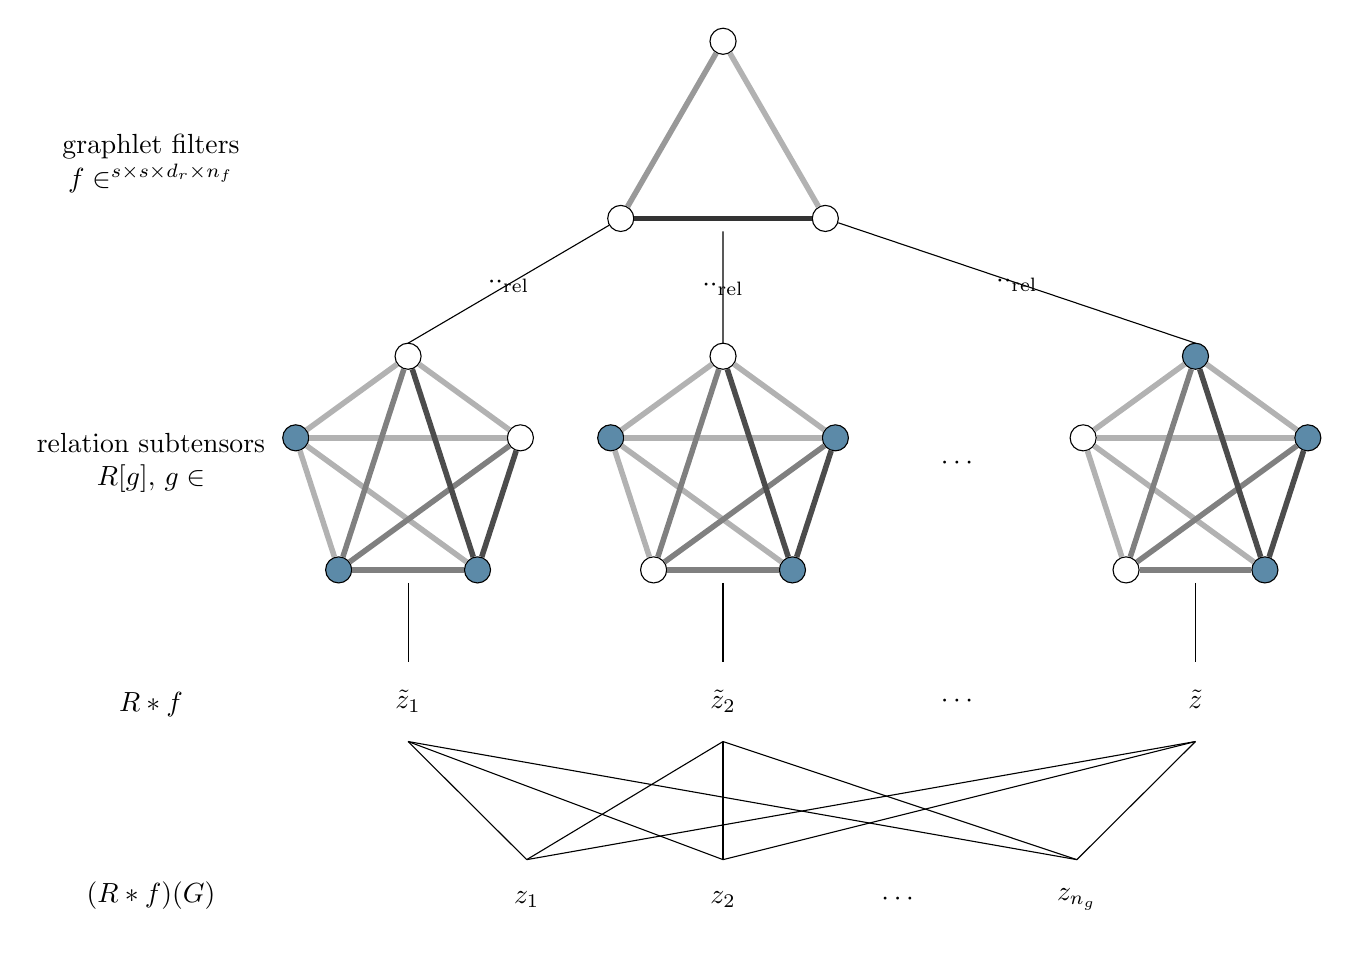
\begin{tikzpicture}[node distance=2cm]


% parameters
\definecolor{highlightcolor}{rgb}{0.36, 0.54, 0.66}
\def\edgethickness{2}
\def\edgeOpacity{{30, 50, 70, 30, 50}}
\def\nodeColors{{"highlightcolor", "highlightcolor", "highlightcolor", "white", "white"}}
\def\graphsize{1.5}

% first graph
\begin{scope}[local bounding box=graph1]
    % Nodes
    \foreach \i in {1,...,5} {
        \pgfmathsetmacro\color{\nodeColors[\i-1]};
        \node[circle, draw, fill=\color] (N1\i) at (90+\i*72:\graphsize) {};
    }

    % Edges
    \foreach \i in {1,...,5} {
        \foreach \j in {1,...,5} {
            \ifnum\i<\j
                \pgfmathtruncatemacro\index{\i-1}
                \pgfmathsetmacro\opacity{\edgeOpacity[\index]}
                \draw[black!\opacity, line width=\edgethickness pt] (N1\i) -- (N1\j);
            \fi
        }
    }
\end{scope}

% second graph
\def\nodeColors{{"highlightcolor", "white", "highlightcolor", "highlightcolor", "white"}}
\begin{scope}[shift={(4,0)}, local bounding box=graph2]
    \foreach \i in {1,...,5} {
        \pgfmathsetmacro\color{\nodeColors[\i-1]};
        \node[circle, draw, fill=\color] (N2\i) at (90+\i*72:\graphsize) {};
    }
    % Edges
    \foreach \i in {1,...,5} {
        \foreach \j in {1,...,5} {
            \ifnum\i<\j
                \pgfmathtruncatemacro\index{\i-1}
                \pgfmathsetmacro\opacity{\edgeOpacity[\index]}
                \draw[black!\opacity, line width=\edgethickness pt] (N2\i) -- (N2\j);
            \fi
        }
    }
\end{scope}

% third graph
\def\nodeColors{{"white", "white", "highlightcolor", "highlightcolor", "highlightcolor"}}
\begin{scope}[shift={(10,0)}, local bounding box=graph3]
    \foreach \i in {1,...,5} {
        \pgfmathsetmacro\color{\nodeColors[\i-1]};
        \node[circle, draw, fill=\color] (N3\i) at (90+\i*72:\graphsize) {};
    }
    % Edges
    \foreach \i in {1,...,5} {
        \foreach \j in {1,...,5} {
            \ifnum\i<\j
                \pgfmathtruncatemacro\index{\i-1}
                \pgfmathsetmacro\opacity{\edgeOpacity[\index]}
                \draw[black!\opacity, line width=\edgethickness pt] (N3\i) -- (N3\j);
            \fi
        }
    }
\end{scope}

% graphlet filter
\def\triangleSize{1.5} % Set the desired size of the triangle
\begin{scope}[shift={(4,4)}, local bounding box=triangle]
    % nodes
    \foreach \i in {1,...,3} {
        \node[circle, draw] (T\i) at (90+\i*120:\triangleSize) {};
    }
    % edges
    \draw[black!80, line width=\edgethickness pt] (T1) -- (T2);
    \draw[black!40, line width=\edgethickness pt] (T1) -- (T3);
    \draw[black!30, line width=\edgethickness pt] (T2) -- (T3);
\end{scope}

\draw (T1) -- (graph1.north) node[midway] {$\iprod{\cdot}{\cdot}_\mathrm{rel}$};
\draw (triangle.south) -- (graph2.north) node[midway] {$\iprod{\cdot}{\cdot}_\mathrm{rel}$};
\draw (T2) -- (graph3.north) node[midway] {$\iprod{\cdot}{\cdot}_\mathrm{rel}$};
\path (graph2.east) -- (graph3.west) node[midway] {$\cdots$};

\node [minimum size=1cm, below=1cm of graph1.south] (tz1) {$\tilde{z}_1$};
\node [minimum size=1cm, below=1cm of graph2.south] (tz2) {$\tilde{z}_2$};
\node [minimum size=1cm, below=1cm of graph3.south] (tzng) {$\tilde{z}_{\abs{\calG}}$};

\draw (graph1.south) -- (tz1.north);
\draw (graph2.south) -- (tz2.north);
\draw (graph3.south) -- (tzng.north);

\node [minimum size=1cm, below right=1.5cm and 1cm of tz1.south] (z1) {$z_1$};
\node [minimum size=1cm, below=1.5cm of tz2.south] (z2) {$z_2$};
\node [minimum size=1cm, below left=1.5cm and 1cm of tzng.south] (zng) {$z_{n_g}$};
\path (tz2.east) -- (tzng.west) node[midway] {$\cdots$};

\draw (tz1.south) -- (z1.north);
\draw (tz1.south) -- (z2.north);
\draw (tz1.south) -- (zng.north);
\draw (tz2.south) -- (z1.north);
\draw (tz2.south) -- (z2.north);
\draw (tz2.south) -- (zng.north);
\draw (tzng.south) -- (z1.north);
\draw (tzng.south) -- (z2.north);
\draw (tzng.south) -- (zng.north);
\path (z2.east) -- (zng.west) node[midway] {$\cdots$};

\node [left=0.1cm of graph1.west, align=center] (relsubtensors) {relation subtensors\\ $R[g],\, g \in \calG$};
\node [left=of tz1, below=6.5em of relsubtensors] (relconv) {$R \ast \bm{f}$};
\node [left=of z1, below=5.25em of relconv] (relconvsoft) {$(R \ast \bm{f})(G)$};
\node [left=of triangle, above=8em of relsubtensors,  align=center] (filters) {graphlet filters \\ $\bm{f} \in \reals^{s \times s \times d_r \times n_f}$};

\end{tikzpicture}
    \caption{A depiction of the graphlet relational convolution operation. The input is a relation tensor $R$ of shape $m \times m \times d_r$, giving pairwise relations of dimension $d_r$ between a sequence of $m$ objects. A graphlet filter of size $s$ is parameterized by a relation tensor of shape $s \times s \times d_r$. The graphlet convolution operation computes relational inner products for each of $n_f$ graphlet filters, $\bm{f}$. This gives a vector representation, $z_i \in \reals^{n_f}$, for each discrete group of $s$ objects. Finally, this is synthesized into a vector representation for each of $n_g$ `soft groups', $G$. The overall operation is denoted by $(z_1, \ldots, z_{n_g}) = (R \ast \bm{f})(G)$.}\label{fig:relconvdiagram}
\end{figure}


\subsection{Relational convolutions with `soft' groups}

In the above formulation, the groups are `discrete', and we consider every possible group. Having discrete groups can be nice for interpretability. But, one challenge we face here is that the number of objects grows rapidly after applying this module. That is, the number of groups to consider $\abs{\calG} = \binom{m}{s}$ may be intractably large, especially if the number of input objects $n$ is large. This may pose computational issues. Furthermore, considering every possible grouping may be unnecessary and may make learning more difficult.

In order to address these issues, we might want to explicitly model the groups. This allows us to control the number of objects in the output sequence such that only useful groups are considered.

In the next section, we outline some ways to model `soft groups' using \textit{Grouping Layers}. These layers take a sequence of objects and/or the relation tensor as input and produce a group matrix $G \in \reals^{m \times n_g}$ representing $n_g$ `soft groups'. The $(i,j)$th entry of the group matrix represents the degree to which the $i$th object belongs to the $j$th group. The number of groups $n_g$ is a configurable hyperparameter of the grouping layers. The groups may be a function of the position of the objects in the sequence, the features of the objects, and/or the relations between objects. Different grouping schemes may be more or less appropriate for different tasks. This is discussed in detail in the next section. For now, we assume that the group matrix $G$ is given as input the relational convolution layer.

Consider the group matrix $G \in \reals^{m \times n_g}$ and filters $\bm{f}$ of size $s$. First, we use $G$ to compute a ``group-match score'' for each discrete group $g$ of size $s$ (e.g., $g \in \calG = \binom{[m]}{s}$). This is done via

\begin{equation}
    \label{eq:group_match_score}
    \begin{split}
        G &\gets \text{SoftPlus}(G)\\
        \alpha_{gk} &\gets \text{Softmax}\paren{\paren{\prod_{i \in g} G[i,k]}_{g \in \calG}}, \quad g \in \calG, k \in [n_g],
    \end{split}
\end{equation}

where the soft-plus function is $\text{Softplus}(x) = \log(\exp(x + 1))$, applied elementwise. This has the effect of making the group matrix $G$ non-negative which is needed for the product of its elements to represent a ``group-match score''. The product inside the softmax is over elements in the discrete group $g \in \calG$. Hence, it will be large whenever the softgroup $G[:, k]$ aligns with the discrete group $g$. Thus, $\alpha_{gk}$ is a normalized ``group-match score'' indicating the degree to which the discrete group $g$ matches the given soft group $G[:,k]$. Note that the group match scores of discrete groups sum to one: $\sum_{g \in G} \alpha_{gk} = 1, \ \forall k \in [n_g]$.

Now, we can define the `soft' relational inner product given the `soft' group $G_k = G[:, k]$ by
\begin{equation}
    \label{eq:soft_relational_inner_prod}
    \langle R, \boldsymbol{f} \, \vert \, G_k \rangle_R \coloneqq \sum_{g \in \calG} \alpha_{gk} \iprod{R[g]}{\boldsymbol{f}}_\mathrm{rel}
\end{equation}

This notation should be read as ``the relational inner product of the relation tensor $R$ with the graphlet filters $\boldsymbol{f}$ given the group $G_k$''. This expression is essentially a convex combination of the relational inner product with all possible discrete groups weighted by how much they match the soft group $G_k$.

With this modification, the number of objects in the output sequence is fixed and controlled by the number of groups, $n_g$ (which is a hyperparameter). The output sequence of the relational convolution given groups $G$ is now given by

\begin{equation}
    \label{eq:soft_relational_convolution_groups}
    (R \ast \bm{f})(G) = \left( \softreliprod{R}{\bm{f}}{G_1}, \ldots, \softreliprod{R}{\bm{f}}{G_{n_g}} \right) \in \left(\mathbb{R}^{n_f}\right)^{n_g}
\end{equation}

\comment{TODO: is this notation good?}

\subsection{Efficiency of `convolutions'}
The operation we have defined here is a `convolution' in the sense that we take a patch of the relation tensor, given by a group, and compare the relations within it to a template graphlet filter via an appropriately-defined inner product. This is similar to how, in a convolutional neural network, we would take a patch of an image and compare it to an image filter. Another similarity to CNNs is that the same graphlet filters are used for all groupings, thus enabling weight-sharing. This is similar to how the same convolutional filters are used for all image patches in a CNN. This makes our framework quite efficient when it comes to the number of parameters and, hopefully, makes learning easier.

% This connection extends to (message-passing) graph neural networks. A key difference however is the following. In a graph neural network, we compute a convolution \textit{along} the graph (i.e.: the graph is what determines a node's neighbors for message-passing). What we are proposing here is that we `convolve' the (relational) graph itself with another graph. 

This analogy motivates one possible style of architectures in our framework~\Cref{fig:relational_framework}. Namely, to have the number of groups after each relational-grouping module decrease while increasing the number of filters. This can be done until we obtain a single group with a long feature vector. This should give a representation of the relational features across all objects, including higher-order relational features (i.e., relations on relations). This single vector can then be passed to a dense feedforward network. This is similar to the ``fully convolutional network'' architecture, where the height and width of the tensor are iteratively decreased (by pooling layers) while increasing the number filters, resulting in a long and thin vector.



% \section{Grouping Layers}\label{sec:grouping_layers}

\textcolor{red}{remove this section if we use the alternate `soft groups' model.}

A grouping layer is a layer which outputs a group matrix $G \in \reals^{m \times n_g}$ representing the degree to which each object $i \in [m]$ belongs to each group $j \in [n_g]$. The number of groups $n_g$ is a configurable hyperparameter. We briefly describe some proposals for grouping layers with different properties.

\textbf{Temporal (Positional) Grouping.} In the temporal grouping layer, the groups are a function only of the temporal order of the objects. This can be achieved by learning the group matrix $G$ directly as a parameter of the model. $G$ will be optimized along with the rest of the model parameters as a function of its effect on the relational convolution layer. Temporal grouping would be appropriate in situations where the order in which objects appear is predetermined and indicates the relevant groups. For example, objects that are positionally close to each other may be grouped together.

\textbf{Feature-based Grouping.} In a feature-based grouping layer, the group(s) to which each object belongs is a function of that object's features (and position). That is,
\begin{equation}\label{eq:feat_grouping}
        G \gets \begin{bmatrix}
            \phi(1, x_1)^\top \\
            \vdots \\
            \phi(m, x_m)^\top
        \end{bmatrix} \in \reals^{m \times n_g},
\end{equation}

\noindent where $\phi: [m] \times \calX \to \reals^{n_g}$ is a learnable function which maps an object's temporal order $i$ and feature representation $x_i$ to a $n_g$-dimensional group membership vector where the $j$th entry of the vector represents the degree to which the object belongs to the $j$th group. For example $\phi$ can be a multi-layer perceptron of the form $\phi(i, x) = \mathrm{MLP}(\mathrm{concat}(e_i, x))$. Feature-based grouping may be useful in situations where group membership can be determined for each object using only that object's features, irrespective of the context of the other objects in the sequence.

\textbf{Context-aware Grouping.} In some applications, the group(s) to which each object belongs to may depend on the full context of the other objects in the sequence. One way to model this is to use a message-passing neural network to update the representations of each object, incorporating the context of the other objects in the sequence. Then, a multi-layer perceptron is applied to each encoded object to produce the group membership vector for that object.
\begin{equation}\label{eq:context_grouping}
    \begin{split}
        E_i &\gets \mathrm{MessagePassing}\paren{x_i, \set{x_1, \ldots, x_m}}, \ i \in [m] \\
        G &\gets \begin{bmatrix}\mathrm{MLP}(E_1)^\top \\ \vdots \\ \mathrm{MLP}(E_m)^\top \end{bmatrix} \in \reals^{m \times n_g}.
    \end{split}
\end{equation}

This is the most general form of grouping, as it encompasses the previous two forms as special cases. The updated representation of each object $E_i$ now contains any relevant information about the other objects which should be considered in computing its group membership vector. One simple and effective option for the message-passing operation is to use self-attention. In this case, since an inner product relation layer precedes the relational convolution layer, the relation tensor can be re-used in the self-attention operation to compute attention scores.

\section{Experiments}\label{sec:experiments}

The \textit{relational games} dataset was contributed as a benchmark for relational reasoning by~\citep{shanahanExplicitlyRelationalNeural}. It consists of a family of binary classification tasks for identifying abstract relational rules between a set of objects represented as images. The objects consist of three sets of simple geometric shapes, referred to as ``pentominoes'', ``hexominoes'', and ``stripes'' (\Cref{fig:relational_games_objects}). The objects are arranged in a $3 \times 3$ grid. Each relational game task corresponds to some relationship between the objects (see~\Cref{tab:relational_games_tasks} and~\Cref{fig:relational_games_tasks}), and the target is to classify whether the relationship holds among a given sequence of objects or not.

In our experiments, we evaluate out-of-distribution generalization by training all models on the pentominoes objects and evaluating on the hexominoes and stripes objects. The input to all models is presented as a sequence of $9$ objects, each represented as a $12 \times 12 \times 3$ RGB image. In all models, the objects are processed independently by a CNN with a shared architecture. This produces a sequence of $9$ $d$-dimensional vectors. The sequence of objects is then passed to the relation-processing component of the model. The results are then flattened and passed through an MLP with a shared architecture to produce the final prediction. We compare four models: a relational convolution model (abbreviated RelConvNet), CoRelNet~\citep{kergNeuralArchitecture2022}, PrediNet~\citep{shanahanExplicitlyRelationalNeural}, and a Transformer~\citep{vaswani2017attention}. The architectural details of each model are described in~\Cref{tab:architectures}.

The pentominoes split of the relational games dataset is used for training. We hold out 1000 samples for validation (during training) and 5000 samples for testing (after training), and use the rest as the training set. The hexominoes and stripes splits are used to test out-of-distribution generalization after training. For each task and model, we train the model for 50 epochs, while tracking training and validation loss and accuracy. We use the categorical cross-entropy loss and the Adam optimizer with learning rate $0.001$, $\beta_1 = 0.9, \beta_2 = 0.999, \epsilon = 10^{-7}$. We use a batch size of 512. For each model and task, we run 5 trials with different random seeds.

\begin{table}[ht]
    \centering
    \begin{tabular}{p{0.2\textwidth}p{0.7\textwidth}}
    \toprule
    Task              & Description                                                                                                                                                                                             \\ \midrule
    \texttt{same}              & Two random cells out of nine are occupied by an object. They are the ``same'' if they have the same color, shape, and orientation (i.e., identical image)                                               \\\hline
    \texttt{occurs}            & The top row contains one object and the bottom row contains three objects. The ``occurs'' relationship holds if at least one of the objects in the bottom row is the same as the object in the top row. \\\hline
    \texttt{xoccurs}           & Same as occurs, but the relationship holds if exactly one of the objects in the bottom row is the same as the object in the top row.                                                                    \\\hline
    \texttt{between}           & The grid is occupied by three objects in a line (horizontal or vertical). The ``between'' relationship holds if the outer objects are the same.                                                         \\\hline
    \texttt{row match pattern} & The first and third rows of the grid are occupied by three objects each. The ``match pattern'' relationship holds if the relation pattern in each row is the same (e.g., AAA, AAB, ABC, etc.)           \\ \bottomrule
\end{tabular}

    \caption{Relational games tasks.}
    \label{tab:relational_games_tasks}
\end{table}

\begin{figure}
    \centering
    \begin{subfigure}[t]{0.37\textwidth}
        \centering
        \includegraphics[width=\textwidth]{figs/relational_games_objects.pdf}
        % \caption{Examples of objects from each split.}
        \label{fig:relational_games_objects}
    \end{subfigure}
    \begin{subfigure}[t]{0.62\textwidth}
        \centering
        \includegraphics[width=\textwidth]{figs/relational_games_tasks.pdf}
        % \caption{Examples of problem instances for each task. The top row is an example where the relation holds and the bottom row is an example where the relation does not hold.}
        \label{fig:relational_games_tasks}
    \end{subfigure}
    \caption{Relational games dataset.~\textbf{Left} Examples of objects from each split.~\textbf{Right} Examples of problem instances for each task. The top row is an example where the relation holds and the bottom row is an example where the relation does not hold.}
    \label{fig:relational_games_dataset}
\end{figure}

\begin{table}[ht]
    \centering
    \input{figs/experiments/architectures_table.tex}
    \caption{Model architectures.}
    \label{tab:architectures}
\end{table}



\begin{figure}
    \centering
    \includegraphics[width=\textwidth]{figs/experiments/all_training_curves.pdf}
    \caption{Training curves for each relational games task. Showing curves up to 2,000 batch steps. Solid lines indicate the mean over 5 trials and the shaded regions indicate a bootstrap 95\% confidence interval.}\label{fig:training_curves}
\end{figure}

\textbf{Sample efficiency.} We observe that the relational inductive biases of RelConvNet, and relational models more generally, grant a significant advantage in sample-efficiency.~\Cref{fig:training_curves} shows the training accuracy over the first 2,000 batches for each model. RelConvNet, CoRelNet, and PrediNet are explicitly relational architectures, whereas the Transformer is not. The Transformer is able to process relational information through its attention mechanism, but this information is entangled with the features of individual objects (which, for these relational tasks, is extraneous information). The Transformer consistently requires the largest amount of data to learn the relational games tasks. PrediNet tends to be more sample-efficient. RelConvNet and CoRelNet are the most sample-efficient, with RelConvNet only slightly more sample-efficient on the `same', `occurs', `xoccurs', and `between' tasks.

On the `match pattern' task, however, RelConvNet is significantly more sample-efficient. We attribute this to the fact that RelConvNet is able to model higher-order relations through its relational convolution module. The `match pattern' task can be thought of as a simple second-order relational tasks---it involves computing relations between two groups objects, and comparing those relations between the two groups. The relational convolution module naturally models this kind of situation since it considers groups of objects and describes the relations between them. The performance we observe here indicates that the relational games dataset is in some sense saturated by models like RelConvNet and CoRelnet and that more complex relational benchmarks are needed to evaluate this class of models. In particular, benchmarks which test the ability to model higher-order relations.

\begin{table}
    \centering
    \begin{tabular}{llll}
\toprule
              &                           &     Hexos Accuracy &   Stripes Accuracy \\
Task & Model &                    &                    \\
\midrule
same & CoRelNet &  $0.988 \pm 0.006$ &  $0.724 \pm 0.112$ \\
              & PrediNet &  $0.990 \pm 0.004$ &  $0.983 \pm 0.007$ \\
              & Transformer &  $0.997 \pm 0.001$ &  $0.993 \pm 0.004$ \\
              & RelConvNet &  $0.989 \pm 0.002$ &  $0.974 \pm 0.003$ \\
              & RelConvNet (Temporal G) &  $0.981 \pm 0.002$ &  $0.965 \pm 0.007$ \\
              & RelConvNet (Feature G) &  $0.985 \pm 0.001$ &  $0.978 \pm 0.006$ \\
              & RelConvNet (Contextual G) &  $0.981 \pm 0.002$ &  $0.969 \pm 0.012$ \\\hline
occurs & CoRelNet &  $0.992 \pm 0.004$ &  $0.518 \pm 0.012$ \\
              & PrediNet &  $0.907 \pm 0.020$ &  $0.775 \pm 0.046$ \\
              & Transformer &  $0.881 \pm 0.015$ &  $0.724 \pm 0.021$ \\
              & RelConvNet &  $0.980 \pm 0.001$ &  $0.880 \pm 0.015$ \\
              & RelConvNet (Temporal G) &  $0.983 \pm 0.001$ &  $0.920 \pm 0.012$ \\
              & RelConvNet (Feature G) &  $0.788 \pm 0.112$ &  $0.747 \pm 0.099$ \\
              & RelConvNet (Contextual G) &  $0.951 \pm 0.004$ &  $0.830 \pm 0.044$ \\\hline
xoccurs & CoRelNet &  $0.980 \pm 0.007$ &  $0.606 \pm 0.035$ \\
              & PrediNet &  $0.872 \pm 0.036$ &  $0.810 \pm 0.028$ \\
              & Transformer &  $0.867 \pm 0.017$ &  $0.753 \pm 0.031$ \\
              & RelConvNet &  $0.967 \pm 0.001$ &  $0.946 \pm 0.006$ \\
              & RelConvNet (Temporal G) &  $0.963 \pm 0.006$ &  $0.939 \pm 0.012$ \\
              & RelConvNet (Feature G) &  $0.760 \pm 0.107$ &  $0.754 \pm 0.103$ \\
              & RelConvNet (Contextual G) &  $0.942 \pm 0.020$ &  $0.901 \pm 0.029$ \\\hline
between & CoRelNet &  $0.995 \pm 0.001$ &  $0.582 \pm 0.063$ \\
              & PrediNet &  $0.978 \pm 0.006$ &  $0.950 \pm 0.019$ \\
              & Transformer &  $0.986 \pm 0.003$ &  $0.961 \pm 0.010$ \\
              & RelConvNet &  $0.991 \pm 0.001$ &  $0.988 \pm 0.002$ \\
              & RelConvNet (Temporal G) &  $0.992 \pm 0.001$ &  $0.979 \pm 0.004$ \\
              & RelConvNet (Feature G) &  $0.993 \pm 0.001$ &  $0.981 \pm 0.003$ \\
              & RelConvNet (Contextual G) &  $0.992 \pm 0.002$ &  $0.972 \pm 0.012$ \\\hline
match pattern & CoRelNet &  $0.942 \pm 0.011$ &  $0.581 \pm 0.026$ \\
              & PrediNet &  $0.710 \pm 0.040$ &  $0.658 \pm 0.053$ \\
              & Transformer &  $0.627 \pm 0.005$ &  $0.591 \pm 0.006$ \\
              & RelConvNet &  $0.961 \pm 0.015$ &  $0.870 \pm 0.041$ \\
              & RelConvNet (Temporal G) &  $0.979 \pm 0.003$ &  $0.967 \pm 0.002$ \\
              & RelConvNet (Feature G) &  $0.976 \pm 0.003$ &  $0.958 \pm 0.009$ \\
              & RelConvNet (Contextual G) &  $0.935 \pm 0.047$ &  $0.896 \pm 0.060$ \\
\bottomrule
\end{tabular}

    \caption{Out-of-distribution Generalization results on relational games. We report means $\pm$ standard error of mean over 5 trials.}\label{tab:ood_generalization}

\end{table}

\begin{figure}
    \begin{subfigure}{0.5\textwidth}
        \centering
        \includegraphics[width=\textwidth]{figs/experiments/hexos_acc.pdf}
        \caption{OoD generalization on Hexos objects}\label{fig:ood_generalization_hexos}
    \end{subfigure}
    \begin{subfigure}{0.5\textwidth}
        \centering
        \includegraphics[width=\textwidth]{figs/experiments/stripes_acc.pdf}
        \caption{OoD generalization on Stripes objects}\label{fig:ood_generalization_stripes}
    \end{subfigure}
    \caption{Out-of-distribution generalization on hold-out object sets. Bar heights indicate the mean over 5 trials and the errror bars indicate a bootstrap 95\% confidence interval.}\label{fig:ood_generalization}
\end{figure}

\textbf{Out-of-distribution generalization}~\Cref{fig:ood_generalization} and~\Cref{tab:ood_generalization} report model performance on the two hold-out object sets after training. On the hexominoes objects, which are similar-looking to the pentominoes objects used for training, RelConvNet and CoRelNet do nearly perfectly. PrediNet and the Transformer do well on the simpler tasks, but struggle with the more difficult `match pattern' task. The stripes objects are visually more distinct from the pentominoes of the training split, making generalization more difficult. We observe an overall drop in performance for all models. The drop is particularly dramatic for CoRelNet\footnote{Unlike~\citep{kergNeuralArchitecture2022}, we do not use temporal context normalization in our experiments. We believe this is the more appropriate choice for evaluating relational architectures such as RelConvNet and CoRelNet since TCN is an added confounder. We discuss this more in~\Cref{sec:tcn_discussion}.}. We conjecture that this is due to CoRelNet's inability to model multi-dimensional relations, necessitating that all relational information is squeezed into a scalar quantity. \texttt{TODO: elaborate or remove this comment?}. The separation between RelConvNet and the other models is largest on the ``match pattern'' task of the stripes split (the most difficult task and the most difficult generalization split). Here, RelConvNet maintain a mean accuracy of 87\% while the other models drop below 65\%. We conjecture that this is due to RelConvNet's natural ability to model such higher-order relations as well as its ability to model multi-dimensional relations.


\section{Discussion}\label{sec:discussion}

\textbf{Summary.} In this paper, we proposed a framework for hierarchical relational representation learning via a novel relational convolution operation. The relational convolution operation we propose here is a `convolution' in the sense that it considers a patch of the relation tensor, given by a group, and compares the relations within it to a template graphlet filter via an appropriately-defined inner product. This is analogous to convolutional neural networks, where we would compare an image filter against different patches of the input image. Since the same graphlet filters are used for all groupings, the relational convolution operation implements a form of \textit{parameter-sharing} which yields improved sample-efficiency and generalization.

An important feature of the relational convolution operation is its \textit{interpretability}. The filters $\bm{f} = (f_1, \ldots, f_{n_f})$ are each a particular pattern of relations between $s$ objects. Each object in the output of a relational convolution $R \ast \bm{f}$ represents the degree to which the relations in the group $g$ match the patterns in each filter. By iteratively applying inner product relation layers and relational convolution layers, we obtain an architecture which naturally models \textit{hierarchical} relations.

\textbf{Limitations and future work.} The tasks considered here are solvable by modeling only second-order relations at most. We observe that the relational convolutional networks architecture saturates the relational games benchmark of~\citep{shanahanExplicitlyRelationalNeural}. While the ``contains set'' task demonstrates a sharp separation between relational convolutional networks and existing baselines, this task too only involves second-order relations, and does not fully test the abilities of the framework. A more thorough evaluation of this architecture, and future architectures for modeling hierarchical relations, would require the development of new benchmark tasks and datasets which involve a larger number of objects and higher-order relations. This is a non-trivial task that we leave for future work.

The experiments considered here are synthetic relational tasks designed for a controlled evaluation. In more realistic settings, we envision relational convolutional networks as modules embedded in a broader architecture. For example, a relational convolutions network can be embedded into an RL agent to enable performing tasks involving relational reasoning. Similarly, the framework can be integrated into a Transformer-based model for general sequence modeling tasks by having the decoder attend to the sequence of relational objects produced by relational convolutions.

% \section*{Broader Impact Statement}
% This work proposes an architectural framework for learning representations of hierarchical relations. In our assessment, the potential societal consequences are not distinctive and do not require detailed discussion here.

% \section*{Code and data}
% Code and experimental logs are available at: \texttt{https://[Anonymized]}


% bibliography
\todo{clean up references and make sure they're consistent. i.e., arxiv papers cited the same way, etc.}
\bibliography{references}
\bibliographystyle{plainnat}
% \bibliographystyle{icml2024}
% \bibliographystyle{unsrtnat}

\clearpage
\newpage
\appendix
\onecolumn

\section{Experiments Supplement}\label{sec:experiments_supplement}

\subsection{Relational Games (\Cref{ssec:exp_relational_games})}

The pentominoes split is used for training, and the hexominoes and stripes splits are used to test out-of-distribution generalization after training. We hold out 1000 samples for validation (during training) and 5000 samples for testing (after training), and use the rest as the training set. We train for 50 epochs using the categorical cross-entropy loss and the Adam optimizer with learning rate $0.001$, $\beta_1 = 0.9, \beta_2 = 0.999, \epsilon = 10^{-7}$. We use a batch size of 512. For each model and task, we run 5 trials with different random seeds.\Cref{tab:relational_games_tasks} contains text descriptions of each task in the relational games dataset in the experiments of~\Cref{ssec:exp_relational_games}.~\Cref{tab:relgames_architectures} contains a description of the architectures of each model (or shared component) in the experiments.
\Cref{tab:ood_generalization} reports the accuracy on the hold-out object sets (i.e., the numbers depicted in~\Cref{fig:ood_generalization} of the main text).

\subsection{SET (\Cref{ssec:experiments_set})}

We train for 100 epochs using the categorical cross-entropy loss and the Adam optimizer with learning rate $0.001$, $\beta_1 = 0.9, \beta_2 = 0.999, \epsilon = 10^{-7}$. We use a batch size of 512. For each model and task, we run 5 trials with different random seeds.\Cref{tab:set_architectures} contains a description of the architecture of each model in the ``contains set'' experiments of~\Cref{ssec:experiments_set}.~\Cref{tab:set_acc} reports the generalization accuracies on the hold-out `sets' (i.e., the numbers depicted in~\Cref{fig:contains_set_acc} of the main text).

\begin{table}[H]
    \centering
    \begin{tabular}{p{0.2\textwidth}p{0.7\textwidth}}
    \toprule
    Task              & Description                                                                                                                                                                                             \\ \midrule
    \texttt{same}              & Two random cells out of nine are occupied by an object. They are the ``same'' if they have the same color, shape, and orientation (i.e., identical image)                                               \\\hline
    \texttt{occurs}            & The top row contains one object and the bottom row contains three objects. The ``occurs'' relationship holds if at least one of the objects in the bottom row is the same as the object in the top row. \\\hline
    \texttt{xoccurs}           & Same as occurs, but the relationship holds if exactly one of the objects in the bottom row is the same as the object in the top row.                                                                    \\\hline
    \texttt{between}           & The grid is occupied by three objects in a line (horizontal or vertical). The ``between'' relationship holds if the outer objects are the same.                                                         \\\hline
    \texttt{row match pattern} & The first and third rows of the grid are occupied by three objects each. The ``match pattern'' relationship holds if the relation pattern in each row is the same (e.g., AAA, AAB, ABC, etc.)           \\ \bottomrule
\end{tabular}

    \caption{Relational games tasks.}\label{tab:relational_games_tasks}
\end{table}

\begin{table}[H]
    \centering
    \begin{tabular}{p{0.25\textwidth}p{0.75\textwidth}}
    \toprule
    Model / Component & Architecture \\ \midrule
    Common CNN \newline Embedder & \texttt{Conv2D} $\to$ \texttt{MaxPool2D} $\to$ \texttt{Conv2D} $\to$ \texttt{MaxPool2D} $\to$ \texttt{Flatten}. \newline
                        \texttt{Conv2D}: num filters = 16, filter size = $3 \times 3$, activation = relu. \newline
                        \texttt{MaxPool2D}: stride = 2. \\\hline
    RelConvNet        & \texttt{CNN} $\to$ \texttt{MD-IPR} $\to$ \texttt{RelConv} $\to$ \texttt{Flatten} $\to$ \texttt{MLP}. \newline
                        \texttt{MD-IPR}: relation dim = 16, projection dim = 4, symmetric. \newline
                        \texttt{RelConv}: num filters = 16, filter size = 3, discrete groups = combinations. \\\hline
    CoRelNet          & \texttt{CNN} $\to$ \texttt{CoRelNet} $\to$ \texttt{Flatten} $\to$ \texttt{MLP}. \newline
                        Standard CoRelNet has no hyperparameters. \\\hline
    PrediNet          & \texttt{CNN} $\to$ \texttt{PrediNet} $\to$ \texttt{Flatten} $\to$ \texttt{MLP}. \newline
                        \texttt{PrediNet}: key dim = 4, number of heads = 4, num relations = 16. \\\hline
    Transformer       & \texttt{CNN} $\to$ \texttt{TransformerEncoder} $\to$ \texttt{AveragePooling} $\to$ \texttt{MLP}. \newline
                    \texttt{TransformerEncoder}: num layers = 1, num heads = 8, feedforward intermediate size = 32, activation = relu. \\\hline
    GCN               &
        \texttt{CNN} $\to$ \texttt{AddPosEmb} $\to$ (\texttt{GCNConv} $\to$ \texttt{Dense}) $\times 2$ $\to$ \texttt{AveragePooling} $\to$ \texttt{MLP}. \newline
        \texttt{GCConv}: channels = 32, \texttt{Dense}: num neurons = 32, activation = relu \\\hline
    GAT               &
        \texttt{CNN} $\to$ \texttt{AddPosEmb} $\to$ (\texttt{GATConv} $\to$ \texttt{Dense}) $\times 2$ $\to$ \texttt{AveragePooling} $\to$ \texttt{MLP}. \newline
        \texttt{GATonv}: channels = 32, \texttt{Dense}: num neurons = 32, activation = relu \\\hline
    GCN               &
        \texttt{CNN} $\to$ \texttt{AddPosEmb} $\to$ (\texttt{GINConv} $\to$ \texttt{Dense}) $\times 2$ $\to$ \texttt{AveragePooling} $\to$ \texttt{MLP}. \newline
        \texttt{GINConv}: channels = 32, \texttt{Dense}: num neurons = 32, activation = relu \\\hline
                Common output MLP & \texttt{Dense(64, `relu')} $\to$ \texttt{Dense(2)}. \\ \bottomrule
\end{tabular}
    \caption{Model architectures for relational games experiments.}\label{tab:relgames_architectures}
\end{table}

\begin{table}[H]
    \centering
    \begin{tabular}{llll}
\toprule
              &                           &     Hexos Accuracy &   Stripes Accuracy \\
Task & Model &                    &                    \\
\midrule
same & CoRelNet &  $0.988 \pm 0.006$ &  $0.724 \pm 0.112$ \\
              & PrediNet &  $0.990 \pm 0.004$ &  $0.983 \pm 0.007$ \\
              & Transformer &  $0.997 \pm 0.001$ &  $0.993 \pm 0.004$ \\
              & RelConvNet &  $0.989 \pm 0.002$ &  $0.974 \pm 0.003$ \\
              & RelConvNet (Temporal G) &  $0.981 \pm 0.002$ &  $0.965 \pm 0.007$ \\
              & RelConvNet (Feature G) &  $0.985 \pm 0.001$ &  $0.978 \pm 0.006$ \\
              & RelConvNet (Contextual G) &  $0.981 \pm 0.002$ &  $0.969 \pm 0.012$ \\\hline
occurs & CoRelNet &  $0.992 \pm 0.004$ &  $0.518 \pm 0.012$ \\
              & PrediNet &  $0.907 \pm 0.020$ &  $0.775 \pm 0.046$ \\
              & Transformer &  $0.881 \pm 0.015$ &  $0.724 \pm 0.021$ \\
              & RelConvNet &  $0.980 \pm 0.001$ &  $0.880 \pm 0.015$ \\
              & RelConvNet (Temporal G) &  $0.983 \pm 0.001$ &  $0.920 \pm 0.012$ \\
              & RelConvNet (Feature G) &  $0.788 \pm 0.112$ &  $0.747 \pm 0.099$ \\
              & RelConvNet (Contextual G) &  $0.951 \pm 0.004$ &  $0.830 \pm 0.044$ \\\hline
xoccurs & CoRelNet &  $0.980 \pm 0.007$ &  $0.606 \pm 0.035$ \\
              & PrediNet &  $0.872 \pm 0.036$ &  $0.810 \pm 0.028$ \\
              & Transformer &  $0.867 \pm 0.017$ &  $0.753 \pm 0.031$ \\
              & RelConvNet &  $0.967 \pm 0.001$ &  $0.946 \pm 0.006$ \\
              & RelConvNet (Temporal G) &  $0.963 \pm 0.006$ &  $0.939 \pm 0.012$ \\
              & RelConvNet (Feature G) &  $0.760 \pm 0.107$ &  $0.754 \pm 0.103$ \\
              & RelConvNet (Contextual G) &  $0.942 \pm 0.020$ &  $0.901 \pm 0.029$ \\\hline
between & CoRelNet &  $0.995 \pm 0.001$ &  $0.582 \pm 0.063$ \\
              & PrediNet &  $0.978 \pm 0.006$ &  $0.950 \pm 0.019$ \\
              & Transformer &  $0.986 \pm 0.003$ &  $0.961 \pm 0.010$ \\
              & RelConvNet &  $0.991 \pm 0.001$ &  $0.988 \pm 0.002$ \\
              & RelConvNet (Temporal G) &  $0.992 \pm 0.001$ &  $0.979 \pm 0.004$ \\
              & RelConvNet (Feature G) &  $0.993 \pm 0.001$ &  $0.981 \pm 0.003$ \\
              & RelConvNet (Contextual G) &  $0.992 \pm 0.002$ &  $0.972 \pm 0.012$ \\\hline
match pattern & CoRelNet &  $0.942 \pm 0.011$ &  $0.581 \pm 0.026$ \\
              & PrediNet &  $0.710 \pm 0.040$ &  $0.658 \pm 0.053$ \\
              & Transformer &  $0.627 \pm 0.005$ &  $0.591 \pm 0.006$ \\
              & RelConvNet &  $0.961 \pm 0.015$ &  $0.870 \pm 0.041$ \\
              & RelConvNet (Temporal G) &  $0.979 \pm 0.003$ &  $0.967 \pm 0.002$ \\
              & RelConvNet (Feature G) &  $0.976 \pm 0.003$ &  $0.958 \pm 0.009$ \\
              & RelConvNet (Contextual G) &  $0.935 \pm 0.047$ &  $0.896 \pm 0.060$ \\
\bottomrule
\end{tabular}

    \caption{Out-of-distribution generalization results on relational games. We report means $\pm$ standard error of mean over 5 trials. These are the numbers associated with~\Cref{fig:ood_generalization}.}\label{tab:ood_generalization}
\end{table}

\begin{table}[H]
    \centering
    \begin{tabular}{p{0.25\textwidth}p{0.75\textwidth}}
    \toprule
    Model / Component & Architecture                                                                                                                                                                                                                                                                                       \\ \midrule
    Common CNN \newline Embedder & \texttt{Conv2D} $\to$ \texttt{MaxPool2D} $\to$ \texttt{Conv2D} $\to$ \texttt{MaxPool2D} $\to$ \texttt{Flatten} $\to$ \texttt{Dense(64, 'relu') $\to$ \texttt{Dense(64, 'tanh')}}. \\
    & \texttt{Conv2D}: num filters = 32, filter size = $5 \times 5$, activation = relu. \\
    & \texttt{MaxPool2D}: stride = 4. \\\hline
    RelConvNet        & \texttt{CNN} $\to$ \texttt{MD-IPR} $\to$ \texttt{RelConv} $\to$ \texttt{Flatten} $\to$ \texttt{MLP}. \\
    & \texttt{MD-IPR}: relation dim = 16, projection dim = 16, symmetric. \\
    & \texttt{RelConv}: num filters = 16, filter size = 3, discrete groups = combinations, symmetric relational inner product with `max' aggregator. \\\hline
    CoRelNet          & \texttt{CNN} $\to$ \texttt{CoRelNet} $\to$ \texttt{Flatten} $\to$ \texttt{MLP}. \\
    & Standard CoRelNet has no hyperparameters. \\\hline
    PrediNet          & \texttt{CNN} $\to$ \texttt{PrediNet} $\to$ \texttt{Flatten} $\to$ \texttt{MLP}. \\
    & \texttt{PrediNet}: key dim = 4, number of heads = 4, num relations = 16. \\\hline
    Transformer       & \texttt{CNN} $\to$ \texttt{TransformerEncoder} $\to$ \texttt{AveragePooling} $\to$ \texttt{MLP}. \\
    & \texttt{TransformerEncoder}: num layers = 1, num heads = 8, feedforward intermediate size = 32, activation = relu. \\\hline
    Common output MLP & \texttt{Dense(64, 'relu')} $\to$ \texttt{Dense(32, 'relu')} $\to$ \texttt{Dense(2)}. \\ \bottomrule
\end{tabular}
    \caption{Model architectures for ``contains set'' experiments.}\label{tab:set_architectures}
\end{table}

\begin{table}[H]
    \centering
    \begin{tabular}{ll}
\toprule
{} &           Accuracy \\
Model       &                    \\
\midrule
RelConvNet  &  $0.979 \pm 0.006$ \\
CoRelNet    &  $0.563 \pm 0.001$ \\
PrediNet    &  $0.508 \pm 0.002$ \\
Transformer &  $0.584 \pm 0.004$ \\
\bottomrule
\end{tabular}

    \caption{Hold-out test accuracy on ``contains set'' task. We report means $\pm$ standard error of mean over 10 trials. These are the numbers associated with~\Cref{fig:contains_set_acc}.}\label{tab:set_acc}
\end{table}
\null
\vfill
\clearpage\newpage
\section{Discussion on use of TCN in evaluating relational architectures}\label{sec:appendix_tcn_discussion}

In~\Cref{ssec:exp_relational_games} the CoRelNet model of~\citet{kergNeuralArchitecture2022} was among the baselines we compared to. In that work, the authors also evaluate their model on the relational games benchmark. A difference between their experimental set up and ours is that they use a method called ``context normalization'' as a preprocessing step on the sequence of objects.

``Context normalization'' was proposed by~\citet{webbLearningRepresentationsThat2020}. The proposal is simple: Given a sequence of objects, $(x_1, \ldots, x_m)$, and a set of context windows $\calW_1, \ldots, \calW_W \subset \set{1, \ldots, m}$ which partition the objects, each object is normalized along each dimension with respect to the other objects in its context. That is, $\paren{z_1, \ldots, z_m} = \mathrm{CN}(x_1, \ldots, x_m)$ is computed as,
\begin{eqnarray*}
    \begin{split}
        \mu_j^{(k)} &= \frac{1}{\abs{\calW_k}} \sum_{t \in \calW_k} (x_t)_j\\
        \sigma_j^{(k)} &= \sqrt{ \frac{1}{\abs{\calW_k}} \sum_{t \in \calW_k} \paren{(x_t)_j - \mu_j^{(k)}}^2 + \varepsilon}\\
        (z_t)_j &= \gamma_j \paren{\frac{(x_t)_j - \mu_j^{(k)}}{\sigma_j^{(k)}}} + \beta_j, \qquad \text{for } t \in \calW_k
    \end{split}
\end{eqnarray*}
where $\gamma = (\gamma_1, \ldots, \gamma_d), \beta = (\beta_1, \ldots, \beta_d)$ are learnable gain and shift parameters for each dimension (initialized at 1 and 0, respectively, as with batch normalization). The context windows represent logical groupings of objects that are assumed to be known. For instance,~\citep{webbEmergentSymbols2021,kergNeuralArchitecture2022} consider a ``relational match-to-sample'' task where 3 pairs of objects are presented in sequence, and the task is to identify whether the relation in the first pair is the same as the relation in the second pair or the third pair. Here, the context windows would be the pairs of objects. In the relational games ``match rows pattern'' task, the context windows would be each row.

It is reported in~\citep{webbEmergentSymbols2021,kergNeuralArchitecture2022} that context normalization significantly accelerates learning and improves out-of-distribution generalization. Since~\citep{webbEmergentSymbols2021,kergNeuralArchitecture2022} use context normalization in their experiments, in this section we aim to explain our choice to exclude it. We argue that context normalization is a confounder and that an evaluation of relational architectures without such preprocessing is more informative.

To understand how context normalization works, consider first a context window of size 2, and let $\beta = 0, \gamma = 1$. Then, along each dimension, we have
\begin{align*}
    % \begin{split}
        \mathrm{CN}(x, x) &= \paren{0, 0},\\
        \mathrm{CN}(x, y) &= \paren{\mathrm{sign}(x - y), \mathrm{sign}(y - x)}.
    % \end{split}
\end{align*}
In particular, what context normalization does when there are two objects is, along each dimension, output 0 if the value is the same, and $\pm 1$ if it is different (encoding whether it is larger or smaller). Hence, it makes the context-normalized output independent of the original feature representation. For tasks like relational games, where the key relation to model is same/different, this preprocessing is directly encoding this information in a ``symbolic'' way. In particular, for two objects $x_1, x_2$, context normalized to produce $z_1, z_2$, we have that $x_1 = x_2$ if and only if $\iprod{z_1}{z_2} = 0$. This makes out-of-distribution generalization trivial, and does not properly test a relational architecture's ability to model the same/different relation.

Similarly, consider a context window of size 3. Then, along each dimension, we have,
\begin{align*}
    % \begin{split}
        \mathrm{CN}(x, x, x) &= \paren{0, 0, 0},\\
        \mathrm{CN}(x, x, y) &= \paren{\frac{1}{\sqrt{2}} \mathrm{sign}(x - y), \frac{1}{\sqrt{2}} \mathrm{sign}(x - y), \frac{1}{\sqrt{2}} \mathrm{sign}(y - x)}.
    % \end{split}
\end{align*}
Again, context normalization symbolically encodes the relational pattern. For any triplet of objects, regardless of the values they take, context normalization produces identical output in the cases above. With context windows larger than 3, the behavior becomes more complex.

These properties of context normalization make it a confounder in the evaluation of relational architectures. In particular, for small context windows especially, context normalization symbolically encodes the relevant information. Experiments on relational architectures should evaluate the architectures' ability to \textit{learn} those relations from data. Hence, we do not use context normalization in our experiments.
\clearpage\newpage
\section{Higher-order relational tasks}

As noted in the discussion, the tasks considered in this paper are solvable by modeling second-order relations at most. One of the main innovations of the relational convolutions architecture over existing relational architectures is its compositionality and ability to model higher-order relations. An important direction of future research is to test the architecture's ability to model hierarchical relations of increasingly higher order. Constructing such benchmarks is a non-trivial task which requires careful thought and consideration. This was outside the scope of this paper, but we provide an initial discussion here which may be useful for constructing such benchmarks in future work.

\textbf{Propositional logic.} Consider evaluating boolean logic formula such as, 
\begin{equation*}
    x_1 \land \paren{(x_2 \lor x_3) \land \paren{(\lnot x_3 \land x_4) \lor (x_5 \land x_6 \land x_7)}}.
\end{equation*}
Evaluating this logical expression (in this form) requires iteratively grouping objects and computing the relations between them. For instance, we begin by computing the relation within $g_1 = (x_3, x_4)$ and the relation within $g_2 = (x_5, x_6, x_7)$, then we compute the relation between the groups $g_1$ and $g_2$, etc. For a task which involves logical reasoning of this hierarchical form, one might imagine the group attention in RelConvNet learning the relevant groups and the relational convolution operation computing the relations within each group. Taking inspiration from logical reasoning with such hierarchical structure may lead to interesting benchmarks of higher-order relational representation.

\textbf{Sequence modeling.} In sequence modeling (e.g., language modeling), modeling the relations between objects is usually essential. For example, syntactic and semantic relations between words are crucial to parsing language. Higher-order relations are also important, capturing syntactic and semantic relational features across different locations in the text and across multiple length-scales and layers of hierarchy~\citep[see for example some relevant work in linguistics][]{frank2012hierarchical,rosario2002descent}. The attention matrix in Transformers can be thought of as implicitly representing relations between tokens. It is possible that composing Transformer layers also learns hierarchical relations. However, as shown in this work and previous work on relational representation, Transformers have limited efficiency in representing relations. Thus, incorporating relational convolutions into Transformer-based sequence models may yield meaningful improvements in the relational aspects of sequence modeling. One way to do this is by cross-attending to a the sequence of relational objects produced by relational convolutions, each of which summarizes the relations within a group of objects at some level of hierarchy.

\textbf{Set embedding.} The objective of set embedding is to map a collection of objects to a euclidean vector which represents the important features of the objects in the set~\citep{zaheer2017deep}. Depending on what the set embedding will be used for, it may need to represent a combination of object-level features and relational information, including perhaps relations of higher order. A set embedder which incorporates relational convolutions may be able to generate representations which summarize relations between objects at multiple layers of hierarchy.

\textbf{Visual scene understanding.} In a visual scene, there are typically several objects with spatial, visual, and semantic relations between them which are crucial for parsing the scene. The CLEVR benchmark on visual scene understanding~\citep{johnson2017clevr} was used in early work on relational representation~\citep{santoroSimpleNeural2017}. In more complex situations, the objects in the scene may fall into natural groupings, and the spatial, visual, and semantic relations between those \textit{groups} may be important for parsing a scene (e.g., objects forming larger components with functional dependence determined by the relations between them). Integrating relational convolutions into a visual scene understanding system may enable reasoning about such higher-order relations.
\clearpage\newpage
\section{Geoemtry of representations learned by MD-IPR and Relational Convolutions}\label{sec:appendix_rep_analysis}

In this section, we explore and visualize the representations learned by MD-IPR and RelConv layers. In particular, we will visualize the representations produced by the RelConvNet model trained on the SET task described in~\Cref{ssec:experiments_set}. Recall that the MD-IPR layer learns encoders $\phi_1, \psi_1, \ldots, \phi_{d_r}, \psi_{d_r}$. In this model $d_r = 16$, $\phi_i = \psi_i$ (so that learned relations are symmetric), and each $\phi_i$ is a linear transformation to $d_{\mathrm{proj}} = 4$-dimensional space. The representations learned by a selection of 6 encoders is visualized in~\Cref{fig:mdirp_encoders_rep}. For each of the 81 possible SET cards, we apply each encoder in the MD-IPR layer, reduce to 2-dimensions via PCA, and visualize how each encoder separates the 4 attributes: number, color, fill, and shape. Observe, for example, that ``Encoder 0'' disentangles color and shape, ``Encoder 2'' disentangles fill, and ``Encoder 3'' disentangles number.

Next, we visualize, we explore the geometry of learned representations of relation vectors. That is, the inner products producing the 16-dimensional relation vector for each pair of objects. For each $\binom{81}{2}$ pairs of SET cards, we compute the 16-dimensional relation vector learned by the MD-IPR layer, reduce to 2 dimensions via PCA, and visualize how the learned relation disentangles the latent same/different relations among the four attributes. This is shown in~\Cref{fig:mdipr_rel_rep}. We see some separation of the underlying same/different relations among the four attributes, even with only two dimensions out of 16.

Finally, we visualize the representations learned by the relational convolution layer. Recall that this layer learns a set of graphlet filters $\bm{f} \in \reals^{s \times s \times d_r \times n_f}$ which form templates of relational patterns against which groups of objects are compared. In our experiments, the filter size is $s = 3$ and the number of filters is $n_f = 16$. Hence, for each group $g$ of 3 SET cards, the relational convolution layer produces a 16-dimensional vector, $\reliprod{R[g]}{\bm{f}} \in \reals^{n_f}$, summarizing the relational structure of the group. Of the $\binom{81}{3}$ possible triplets of SET cards, we create a balanced sample of ``sets'' and ``non-sets''. We then compute $\reliprod{R[g]}{\bm{f}}$ and reduce to 2 dimensions via PCA.~\Cref{fig:conv_rep} strikingly shows that the representations learned by the relational convolution layer very clearly separate triplets of cards which form a set from those that don't form a set.


\begin{figure}
    \centering
    \includegraphics[width=0.9\textwidth]{figs/representation_analysis/mdipr_encoders_rep.pdf}
    \caption{The encoders learned in the MD-IPR layer represent the latent attributes in the SET cards, with different encoders seemingly specializing to encode one or two attributes.}\label{fig:mdirp_encoders_rep}
\end{figure}

\begin{figure}
    \centering
    \includegraphics[width=0.95\textwidth]{figs/representation_analysis/mdipr_rel_rep.png}
    \caption{The relations learned by the MD-IPR layer encodes the latent relations underlying the SET task.}\label{fig:mdipr_rel_rep}
\end{figure}

\begin{figure}
    \centering
    \includegraphics{figs/representation_analysis/conv_rep.pdf}
    \caption{The relational convolution layer produces representations which separates `sets' from `non-sets'.}\label{fig:conv_rep_appdx}
\end{figure}

% \null
% \vfill



\end{document}